% Copyright (C) 2010,2011,2012,2013,2014 The ESPResSo project
%  
% This file is part of ESPResSo.
%   
% ESPResSo is free software: you can redistribute it and/or modify it
% under the terms of the GNU General Public License as published by the
% Free Software Foundation, either version 3 of the License, or (at your
% option) any later version.
%  
% ESPResSo is distributed in the hope that it will be useful, but
% WITHOUT ANY WARRANTY; without even the implied warranty of
% MERCHANTABILITY or FITNESS FOR A PARTICULAR PURPOSE.  See the GNU
% General Public License for more details.
%  
% You should have received a copy of the GNU General Public License
% along with this program.  If not, see <http://www.gnu.org/licenses/>.
%

\chapter{Object-in-fluid}
\label{sec:oif}
\newescommand{oif}

\begin{citebox}
  Please cite~\citewbibkey{cimrak} if you use the object-in-fluid implementation described below. For more details also see the documentation at http://cell-in-fluid.fri.uniza.sk/oif-documentation or contact the Cell-in-fluid Research Group at University of \v Zilina.
\end{citebox}

Simulations using \es work mostly with objects (molecules, atoms, polymers, colloids, crystals, \dots) that are physically composed of points linked together with bonds. These objects are like skeletons, without inner or outer volume. 

The idea behind this module, is to use \es for objects that do have inner volume, for example blood cells, magnetic beads, capsules, \dots The boundary of an object is covered with triangular mesh. The vertices of the mesh are declared in \es as particles. The edges of the mesh define elastic forces keeping the shape of the object. The movement of object is achieved by adding forces to the mesh points.

Modelled elastic or rigid objects are immersed in the LB fluid flow. The fluid interacts with an elastic object resulting in its deformation; this immediately generates forces acting back on the fluid. The aim is to describe the immersed object using the notion of particles, and to create bonds between these particles representing elastic or rigid forces.

The objects are composed of a membrane encapsulating the fluid inside the object. For now, the inside fluid must have the same density and viscosity as the outside fluid. The object is represented by its membrane (boundary), that is discretized using a triangulation. Such triangulation defines interacting particles distributed on the surface of the immersed object \cite{dupin07}:

\begin{itemize}
\item between two particles, corresponding to the edges in the triangulation (modelling the stretching of the membrane), 
\item between three particles, corresponding to the triangles of the triangulation (local area, or local surface preservation of the membrane), 
\item between four particles, corresponding to two triangles from the triangulation sharing a common edge (bending of the membrane). 
\end{itemize}

The object immersed  in the fluid moves under the influence of the deforming forces, defined through the bonds, and under the influence of the fluid motion. This interaction is based on the frictional force between the fluid and the surface particles. Therefore the object moves in the flow only if there is a nonzero difference between the fluid velocity and the particle velocity. In other words, there has to be at least small flow through the membrane, which is in most cases unphysical. However, this unphysical flow through the membrane is probably negligible in larger scales.

\section{Membranes}
With this approach, it is easy to model also elastic sheets, or free membranes that do not necessarily enclose a 3D object. In this case, area\_{}force\_{}global and volume\_{}force interactions are not needed, since these two interactions are meant for closed immersed objects.

\section{Parameters}
There are several parameters involved in this model. All of them should be calibrated according to the intended application. 
\begin{itemize}
\item Mass of the particles. Every particle has its mass, which influences the dynamics. 
\item Friction coefficient. The main parameter describing the fluid-particle interaction is the \verb friction \ parameter from the \es command \verb lbfluid .
\item Parameters of elastic moduli. Elastic behaviour can be described by five different elastic moduli: hyperelastic stretching, bending, local and global area preservation and volume preservation. Each of them has its own scaling parameter: $ks, kb, kal, kag, kv$. Their mathematical formulations have been taken from \cite{dupin07}.
\end{itemize}
The mass of the particles and the friction coefficient can be calibrated using the drag coefficients of the ellipsoidal objects. These drag coefficients have known analytical values and the mass and friction can be calibrated to fit this values. More details about the calibration can be found in \cite{cimrak}.

The elastic parameters are specific to the immersed objects. They correspond to their physical values. More details about their mechanical and biological meaning is presented in \cite{dao03} specifically for red blood cells. However, the proper calibration to fit the experimental data has been performed in \cite{cimrak}.

\section{Geometry}
The membrane of the immersed object is triangulated. In doc/tutorials/03-object\_in\_fluid you can find an example using deformable objects in the fluid.
\begin{center}
  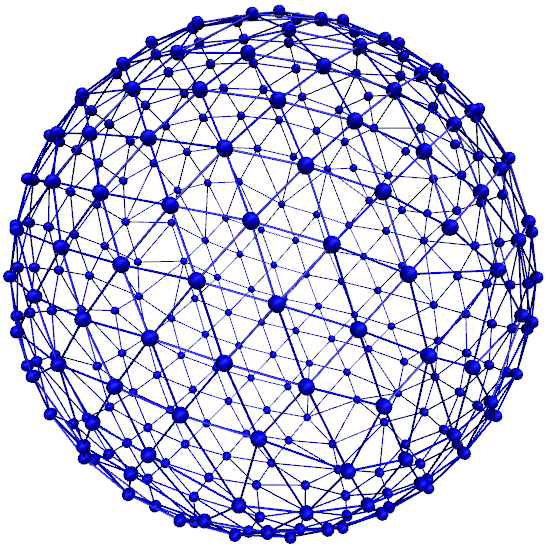
\includegraphics[width=3cm]{figures/oif.png}
\end{center}
Triangulation can be obtained using various software tools. Two files are needed for mesh input: \verb mesh-nodes.dat \ and \verb mesh-triangles.dat . The parameters of the mesh are the number of particles on the surface of the immersed object, denoted by \verb mesh_nnode , and the number of triangular faces in the triangulation, denoted by \verb mesh_ntriangle . These parameters are obtained automatically from \verb mesh-nodes.dat \ and \verb mesh-triangles.dat by counting the number of lines in respective files. 

The \verb mesh-nodes.dat \ thus contains \verb mesh_nnode \ lines with three real numbers separated by blank space, representing three coordinates of the corresponding particle. The membrane is thus discretized into \verb mesh_nnode \ particles with IDs starting from 0 to \verb mesh_nnode-1 . The IDs are assigned in the same order as in the \verb mesh-nodes.dat \ file. 

The \verb mesh-triangles.dat \ contains \verb mesh_ntriangle \ lines with three nonnegative integers separated by blank space. Each line represents one triangle in the triangulation. For algorithmic purposes it is crucial to have defined a correct orientation of the triangle. The orientation is defined using the normal vector associated with the triangle. The important rule is that the normal vector of the triangle must point inside the immersed object.

As an example, let us have one line in the file \verb mesh-triangles.dat \ with numbers 4, 0 and 7. This means that particles with IDs 4, 0 and 7 form one triangular face of the triangulation. The orientation is defined as follows: create two vectors $v_1$ and $v_2$, such that $v_1$ is pointing from particle 4 to particle 0, and $v_2$ is pointing from particle 4 to particle 7. Be careful, the order of vectors and particles matters!

The normal vector $n$ is computed as a vector product $v_1 \times v_2$. The direction of $n$ can be determined by the rule of right hand: the thumb points in the $v_1$ direction, the index finger in the $v_2$ direction and the middle finger in the $n$ direction. Following this principle, all the lines in the \verb mesh-triangles.dat \ files must be such that the normal vectors of the corresponding triangles points inside the immersed object.

These two files are sufficient to describe the geometry and topology of the triangulation. The following geometric entities are necessary for the definition of bonded interactions: position of the particles, edges, lengths of the edges,  triangles, areas of triangles, angles between two triangles sharing a common edge, surface of the immersed object, volume of the immersed object. All these geometrical entities can be computed using the information from the files \verb mesh-nodes.dat \ and \verb mesh-triangles.dat \ and the computation is done in the script \verb scripts/object_in_fluid.tcl .

The script \verb scripts/object_in_fluid.tcl \  reads both mesh files, generates list of edges, and computes all geometrical entities needed for definition of bonded interactions. It then executes commands creating the particles, interactions and bonds.An example of \verb part \ command is as follows:
\begin{verbatim} part 0 pos 3.0 3.0 6.0 type 1 mol 1 mass 1 \end{verbatim}

Note, the is feature \verb mol \ that used for the particles. We use this feature we distinguish between different objects. The upper limit for the number of objects is 10000. However it can be increased by changing the \verb MAX_OBJECTS_IN_FLUID \ constant. 

The following example shows an interaction.   
\begin{verbatim} inter 106 stretching_force 4.6 5.0 \end{verbatim}
This command ("invisible" for the user who executes the \verb scripts/object_in_fluid.tcl \ script) creates an interaction for stretching with ID 106. Detailed description of the available types of interactions is presented in Section \ref{sec:inter-bonded-oif}.

\section{Available commands} 
In order to use the object-in-fluid (OIF) commands and work with immersed objects, the following \es features need to be compiled in: \verb MASS, \ \verb EXTERNAL_FORCES . We do not specifically require \verb LB, \ \verb LB_BOUNDARIES, \ \verb CONSTRAINTS, \ \verb SOFT_SPHERE, \ \verb AREA_FORCE_GLOBAL, \ \verb VOLUME_FORCE . They are most likely to be used (for objects immersed in fluid and interacting with boundaries and each other), but they are not necessary for the following commands. For up-to-date overview of available oif commands see the OIF user guide at cell-in-fluid.fri.uniza.sk/oif-documentation.

\subsection{\label{ssec:oif-init}Initialisation}

\begin{essyntax}
  oif_init
\end{essyntax}
Must be used before any other OIF command, initializes all global variables and lists, does not take any arguments.

\subsection{\label{ssec:oif-info}Information about object-in-fluid structures}

\begin{essyntax}
	oif_info
\end{essyntax}
Prints information about whole framework, \eg all global variables, currently available templates and objects, etc. Does not take any arguments.

\subsection{\label{ssec:oif-create-template}Templates for objects}

\begin{essyntax}
  \require{1,2}{oif_create_template}
  template-id  \var{tid}
  nodes-file  \var{nodes.dat}
  triangles-file  \var{triangles.dat}
  \opt{stretch \var{x} \var{y} \var{z}}
  \opt{ks \var{ks\_value}}
  \opt{kb \var{kb\_value}} 
  \opt{kal \var{kal\_value}}
  \require{3}{\opt{kag \var{kag\_value}}}
  \require{4}{\opt{kv \var{kv\_value}}}
  \begin{features}
  \required[1]{MASS}
  \required[2]{EXTERNAL_FORCES}
  \required[3]{AREA_FORCE_GLOBAL}
  \required[4]{VOLUME_FORCE}
  \end{features}
\end{essyntax}

This command creates a template that will be used for all objects that share the same elastic properties and have the same triangulation.

\begin{arguments}
\item[\var{tid}] specifies a unique ID for each template. The first template has the ID 0. The following ones need to be be numbered consecutively.
\item[\var{nodes.dat}] input file, each line contains three real numbers. These are the $x, y, z$ coordinates of individual surface mesh nodes of the objects.
\item[\var{triangles.dat}] input file, each line contains three integers. These are the ID numbers of the mesh nodes as they appear in \var{nodes.dat}. Note, the first node has ID 0.
\item[\opt{stretch \var{x} \var{y} \var{z}}] coefficients by which the coordinates stored in \var{nodes.dat} will be stretched in the $x, y, z$ direction. The default values are 1.0 1.0 1.0.
\item[\opt{ks \var{ks\_value}}] elastic modulus for stretching forces
\item[\opt{kb \var{kb\_value}}] elastic modulus for bending forces
\item[\opt{kal \var{kal\_value}}] elastic modulus for local area forces
\item[\opt{kag \var{kag\_value}}] elastic modulus for global area forces
\item[\opt{kv \var{kv\_value}}] elastic modulus for volume forces
\end{arguments}

The three switches \verb|ks|, \verb|kb| and \verb|kal| set elastic parameters for local interactions - \verb|ks| for edge stiffness, \verb|kb| for angle preservation stiffness and \verb|kal| for triangle surface preservation stiffness. This stiffness can be either uniform over the whole object, or non-uniform. In case of stretching modulus, we can have spring stiffness the same for all edges in the whole object, or we can choose the value for every edge of the object separately. Analogically, for \verb|kal| and \verb|kb|. Therefore, there are two options for setting \verb|ks|, \verb|kal| and \verb|kb| stiffness. Here is the explanation for \verb|ks|:
\begin{itemize}
\item {\bf Uniform stiffness:} To set uniform stiffness for all edges in the object, use \verb|ks| \var{ks\_value}
\item {\bf Non-uniform stiffness:} To set non-uniform stiffness, prepare a file \var{filename} with number of lines equal to the number of edges of the triangulation. Each line should contain a real number between 0 and 1, so called "weight". Then call
\verb|ks| \var{filename} \var{ksMin} \var{ksMax}
This command reads the weights $weight_i$ for each edge and the stiffness for that edge is set to 
$$
ks_i = ksMin * (1 - weight_i) + ksMax*(weight_i)
$$
For bending stiffness, \var{filename} must contain the same number of lines as there are edges in the object. However, for local area preservation, the stiffness constant is linked to triangles. Therefore, \var{filename} must contain the same number of lines as there are triangles in the object.
\end{itemize}

\warning{At least one elastic modulus needs to be set for the object.} 

\subsection{\label{ssec:oif-add-object}Elastic objects}

\begin{essyntax}
  \require{1,2, possibly 3 or 4}{oif_add_object}
  object-id  \var{oid}
  template-id  \var{tid}
  origin \var{x} \var{y} \var{z}
  part-type \var{type}
  \opt{rotate \var{x} \var{y} \var{z}}
  \opt{mass \var{m}}
  \begin{features}
  \required[1]{MASS}
  \required[2]{EXTERNAL_FORCES}
  \required[3]{AREA_FORCE_GLOBAL}
  \required[4]{VOLUME_FORCE}
  \end{features}
\end{essyntax}

Using a previously defined template \var{tid}, this command creates a new object. Features \verb|AREA_FORCE_GLOBAL| and \verb|VOLUME_FORCE| are needed, if the template used the corresponding elastic moduli.

\begin{arguments}
\item[\var{oid}] unique ID for each object, the first object has the ID 0. The following ones should be numbered consecutively.
\item[\var{tid}] object will be created using nodes, triangle incidences, elasticity parameters and initial stretching saved in this template.
\item[origin \var{x} \var{y} \var{z}] center of the object will be at this point.
\item[part-type \var{type}] can be any integer starting at 0. All particles of one object have the same \verb|part-type|. One can have more objects with the same type of particles, but this is not recommended, because the interactions between objects are set up using these types.
\item[\opt{rotate \var{x} \var{y} \var{z}}] angles in radians, by which the object is initially rotated around the $x, y, z$ axis. Default values are 0.0 0.0 0.0.
\item[\opt{mass \var{m}}] mass of one particle. Default value is 1.0
\end{arguments}

\subsection{\label{ssec:oif-mesh-analyze}Mesh analysis}

\begin{essyntax}
  oif_mesh_analyze
  nodes-file  \var{nodes.dat}
  triangles-file  \var{triangles.dat}
  \opt{orientation}
  \opt{repair \var{output\_file.dat} \var{method}}
  \opt{shift-node-ids \var{output\_file.dat}}
\end{essyntax}

This command is useful for some preparatory work with mesh before it is used for creating elastic objects.

\begin{arguments}
\item[nodes-file \var{nodes.dat}] - file with coordinates of the mesh nodes. The center of the object should be as close to (0,0,0) as possible.
\item[triangles-file \var{triangles.dat}] - file with incidences for all triangles. Each line of this file contains three integer IDs (starting from 0) with indices of three vertices forming one triangle.
\item[\opt{orientation}] checks whether all triangles of the surface mesh are properly oriented. For now, only works for convex (or almost convex) objects.
\item[\opt{repair \var{output\_file.dat} \var{method}}] outputs the corrected \var{triangles.dat} file into \var{output\_file.dat}. For now, only works for convex (or almost convex) objects. \var{method} needs to be set to 1.
\item[\opt{shift-node-ids \var{output\_file.dat}}] subtracts 1 from all numbers in \var{triangles.dat} and saves a new file \var{output\_file.dat}. This is useful, if the mesh generating software starts numbering the particles from 1 instead of 0.
\end{arguments}
	 
\subsection{\label{ssec:oif-object-output}Output information about specific object}

\begin{essyntax}
  \require{1,2, possibly 3 or 4}{oif_object_output}
  object-id  \var{oid}
  \opt{vtk-pos \var{output\_file1.dat}}
  \opt{vtk-pos-folded \var{output\_file2.dat}}
  \opt{vtk-aff \var{output\_file3.dat}}
  \opt{mesh-nodes \var{output\_file4.dat}}
  \begin{features}
  \required[1]{MASS}
  \required[2]{EXTERNAL_FORCES}
  \required[3]{AREA_FORCE_GLOBAL}
  \required[4]{VOLUME_FORCE}
  \end{features}
\end{essyntax}

This command is used to output information about the object that can be used for visualisation or as input for other simulations.

\begin{arguments}
\item[\var{oid}] - the id of the object
\item[\opt{vtk-pos \var{output\_file1.dat}}] outputs the mesh of the object to the desired \var{output\_file1.dat}. Paraview can directly visualize this file.
\item[\opt{vtk-pos-folded \var{output\_file2.dat}}] the same as the previous option, however the whole object is shift such that it is visualized within the simulation box. 
This option is useful for simulating periodical processes when objects flowing out on one side of simulation box are transferred to the opoosite side.
\item[\opt{vtk-aff \var{output\_file3.dat}}] outputs affinity bonds that are currently activated. If no bonds are present, the file will be generated anyway with no bonds to visualize. Paraview can directly visualize this file.
\item[\opt{mesh-nodes \var{output\_file4.dat}}] outputs the positions of the mesh nodes to \var{output\_file4.dat}. In fact, this command creates a new \var{nodes.dat} file that can be used by \verb|oif_object_set|. The center of the object is located at point (0,0,0). This command is aimed to store the deformed shape in order to be loaded later.
\end{arguments}

\subsection{\label{ssec:oif-object-analyze}Descriptive information about specific object}

\begin{essyntax}
  \require{1,2, possibly 3 or 4}{oif_object_analyze}
  object-id  \var{oid}
  \opt{origin}
  \opt{pos-bounds \var{bname}}
  \opt{approx-pos}
  \opt{volume}
  \opt{surface-area}
  \opt{velocity}
  \opt{elastic-forces \var{name(s)} \var{output\_file.dat}}
  \opt{f-metric \var{name}}
  %\opt{affinity \var{name}}
  \begin{features}
  \required[1]{MASS}
  \required[2]{EXTERNAL_FORCES}
  \required[3]{AREA_FORCE_GLOBAL}
  \required[4]{VOLUME_FORCE}
  \end{features}
\end{essyntax}

This command is used to output information about the properties of the object. Some of these properties can also be visualized.
 
\begin{arguments}
\item[\var{oid}] - the id of the object
\item[\opt{origin}] - outputs the location of the center of the object
\item[\opt{pos-bounds \var{bname}}] computes six extremal coordinates of the object. More precisely, runs through the all mesh points and remembers the minimal and maximal $x$-coordinate, $y$-coordinate and $z$-coordinate. If \var{bname} is one of these: \textit{z-min, z-max, x-min, x-max, y-min, y-max} then the procedure returns one number according to the value of \var{bname}. If \var{bname} is \var{all}, then the procedure returns a list of six numbers, namely \textit{x-min, x-max, y-min, y-max, z-min, z-max}.
\item[\opt{approx-pos}] - outputs the approximate location of the center of the object. It is computed as average of 6 mesh points that have extremal $x$, $y$ and $z$ coordinates at the time of object loading.
\item[\opt{volume}] - outputs the current volume of the object
\item[\opt{surface-area}] - outputs the current surface of the object
\item[\opt{velocity}] - outputs the current average velocity of the object. Runs over all mesh points and calculates their average velocity.
\item[\opt{elastic-forces \var{name(s)} \var{output\_file.dat}}] (example \verb|elastic-forces| \var{kv} \var{kb} \var {ks} \var {out.vtk}) - name(s) can be one to five of the following: \var{ks, kb, kal, kag, kv}, in any order. Arguments cannot repeat. Corresponding forces are computed for each node by summing up all contributions.  This computation can be considered as a simple approach to elastic energy evaluation. If the output file has an extension .vtk, a vtk file is written with a scalar data fields that can be visualized in ParaView to show the color coded force magnitudes on the surface of the object. If more than one options were given, one can switch between the visualizations in ParaView. If the file has any other extension (.txt, .dat, \dots) a data file is written with magnitudes of resulting forces in each node (five columns - some of them will be zero, if not all arguments were given).
\item[\opt{f-metric \var{name}}] name can be one of the following: \var{ks, kb, kal, kag, kv}. There is no \var{output\_file} as a second argument for these, because the output is just one number - fmetric/"naive energy" computed as a sum of magnitudes of respective elastic forces over all nodes of the object.
%\item[\opt{affinity \var{name}}] analyzes the affinity-related features: \var{all} prints all following information; \var{nbonds} prints number of currently existing bonds, \textit{aver-bond-length} prints the average bond length of existing bonds; \textit{min-bond-length} prints the length of the minimal bond; \textit{max-bond-length} prints the length of the maximal bond, \textit{min-x-bond} detects the bond with the minimal $x$-coordinate of its bond site and prints this $x$-coordinate; \textit{max-x-bond} - detects the bond with the maximal $x$-coordinate of its bond site and prints this $x$-coordinate.
\end{arguments} 

\subsection{\label{ssec:oif-object-set}Setting properties for specific object}

\begin{essyntax}
  \require{1,2, possibly 3 or 4}{oif_object_set}
  object-id  \var{oid}
  \opt{force \var{x} \var{y} \var{z}}
  \opt{origin \var{x} \var{y} \var{z}}
  \opt{mesh-nodes \var{mesh\_nodes.dat}}
  \opt{kill-motion}
  \opt{un-kill-motion}
  \begin{features}
  \required[1]{MASS}
  \required[2]{EXTERNAL_FORCES}
  \required[3]{AREA_FORCE_GLOBAL}
  \required[4]{VOLUME_FORCE}
  \end{features}
\end{essyntax}

This command sets some properties of the object.

\begin{arguments}
\item[\var{oid}] - the id of the object
\item[\opt{force \var{x} \var{y} \var{z}}] - sets the force vector (\var{x, y, z}) to all mesh nodes of the object. Setting is done using \es command \verb|part $i set ext_force| \var{\$x} \var{\$y} \var{\$z}. Note, that this command sets the external force in each integrate step. So if you want to use the external force only in one iteration, you need to set zero external force in the following integrate step
\item[\opt{origin \var{x} \var{y} \var{z}}] - moves the object so that the origin has coordinates \var{(x, y, z)}
\item[\opt{mesh-nodes \var{mesh\_nodes.dat}}] - deforms the object such that its origin stays unchanged, however the relative positions of the mesh points are taken from file \var{mesh\_nodes.dat}. The file \var{mesh\_nodes.dat} should contain the coordinates of the mesh points with the origin's location at (0,0,0). The procedure also checks whether number of lines in the \var{mesh\_nodes.dat} file is the same as the number of triangulation nodes of the object.
\item[kill-motion] - stops all the particles in the object (analogue to the \verb|part | \var{pid} \verb|fix 1 1 1| command for single particles).
\item[un-kill-motion] - releases the particles in the object (analogue to the \verb|part | \var{pid} \verb| unfix| command for single particles).
\end{arguments} 


%%% Local Variables:
%%% mode: latex
%%% TeX-master: "oif"
%%% End:
